% !TEX root = sum1.tex
\section{Introduction}
Governments worldwide have been faced with the challenge of reducing the spread of Covid-19 while minimizing the economic impact. Social distancing has been widely implemented as the most effective non-pharmaceutical treatment to reduce the health effects of the virus. 
This website records a timeline of Covid-19 and the relevant epidemic prevention measures\cite{Covid19Timeline}. For instance, in March 2020, the Hong Kong government implemented restrictive measures such as banning indoor and outdoor gatherings of more than four people, requiring restaurants to operate at half capacity. As the epidemic worsened, the government tightened measures by limiting public gatherings to two people per group in July 2020. As the epidemic subsided, the Hong Kong government gradually relaxed social distancing restrictions, allowing public group gatherings of up to four people in September 2020. In October 2020, pubs were allowed to serve up to four people per table, and restaurants could serve up to six people per table. Specifically, the Hong Kong government also implemented different measures in different venues \cite{Gov202209}. For example, the catering businesses will have different social distancing requirements depending on their mode of operation for dine-in services. They can operate at 50\%, 75\%, or 100\% of their normal seating capacity at any one time, with a maximum of 2, 2, or 4 people per table, respectively. Bars and pubs may open with a maximum of 6 persons per table and a total number of patrons capped at 75\% of their capacity. The restrictions on the number of persons allowed in premises such as cinemas, performance venues, museums, event premises, and religious premises will remain at 85\% of their capacity.

The measures announced by the Hong Kong government mainly focus on limiting the number of people in each group and the seat occupancy rate. However, implementing these policies in operations can be challenging, especially for venues with fixed seating layouts. In our study, we will focus on addressing this challenge in commercial premises, such as cinemas and music concert venues. We aim to provide a practical tool for venues to optimize seat assignments by proposing a seat assignment policy that takes into account social distancing requirements and the given seat layout. We strive to enable venues to implement social distancing measures effectively by offering a solution that provides specific seating arrangements.


% \subsection{Seat Planning and Seat Assignment}

% According to the social distancing requirement imposed by the government, the size of the largest group is confined, people in the same group can sit together and the adjcent groups should keep distance with each other.

To avoid confusion, we clarify the distinction between `seat planning' and `seat assignment' which will be used in the following parts. In our context, the seat planning means the seat partition in the planning. The planning can be altered later when the planned seats don't match with the size of a coming group or when the seat planning is disrupted after assigning a coming group. In the seat assignment, for the coming group, when accepting it, we assign the seats to the group, and the seats will not be used by others in the future.

% It includes two forms, fixed seat planning and flexible seat planning. The former one is that some seats are unavailable, they may be dismantled or disabled by staff beforehand. The latter one represents the current seat planning, but the planning can be altered later when the planned seats don't match with the size of a coming group or when the seat planning is disrupted after assigning a coming group. 

The following figures illustrate the seat planning and seat assignment. 
% there are two rows for the seat planning. The cross square seats are occupied. 


\begin{figure}[htbp]
    \centering
    \begin{minipage}[t]{0.48\textwidth}
    \centering
    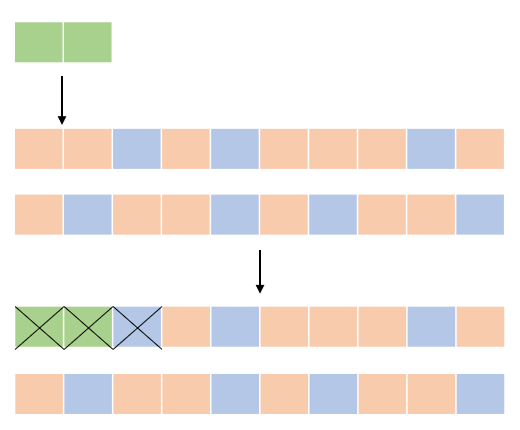
\includegraphics[width=5cm]{./Figures/seat_assign1.png}
    \caption{Assign The Group in Row 1}
    \end{minipage}
    \begin{minipage}[t]{0.48\textwidth}
    \centering
    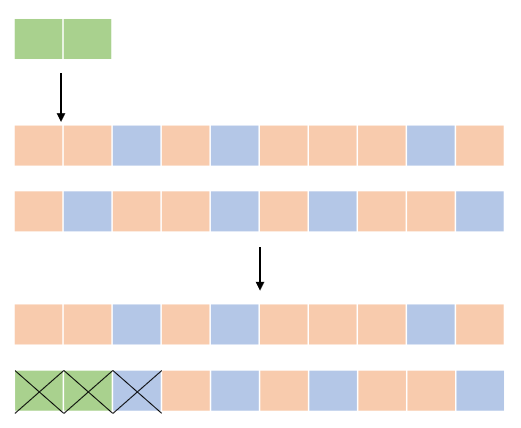
\includegraphics[width=5cm]{./Figures/seat_assign2.png}
    \caption{Assign The Group in Row 2}
    \end{minipage}
\end{figure}

We consider to obtain the seat planning with deterministic and stochatic demand. For the deterministic situation, we have complete and accurate information about the demand for seating. We aim to provide a seat planning that maximizes the number of people accommodated. This situation is applicable in venues like churches or company meetings, where fixed seat layouts are available, and the goal is to assign seats to accommodate as many people as possible within the given layout.

% This situation corresponds to the basic problem of assigning more people with the fixed seat layout, such as in a church, a company meeting. It applies in the place where the seat has been provided in advance in case people don;t follow the rules.

For the stochastic situation, we have knowledge of the demand distribution before the actual demand is realized. We aim to generate a seat planning that maximizes the expected number of people accommodated. This approach is suitable for venues where seats have been pre-allocated to ensure compliance with social distancing rules. By considering the demand distribution, we can optimize the seat planning to accommodate the maximum number of people while maintaining social distancing.

Regarding the seat assignment, we consider the dynamic demand based on the seat planning. For the dynamic situation, the decision to accept or reject a group is made for each incoming group. This situation is commonly encountered in venues such as cinemas or music concerts, where decisions can be made on a group-by-group basis. The goal is to make timely decisions regarding seat assignments, considering factors such as available seating capacity, social distancing requirements and the specific size of each group.

% based on specific requirements. According to the different requirements, we can assign the seats in two forms. Under the fixed seat planning, the fixed seats will be disabled beforehand in case someone don't obey the social distancing rule. Under the flexible seat planning, we can allocate seats immediately upon arrival or at a later time. 


% To avoid confusion regarding the terms `seat planning' and `seat assignment', it is important to clarify the distinction between them. In our context, seat planning involves determining the arrangement of seats within a venue or space based on the size or layout of the room. This includes deciding on seats partition with social distancing. On the other hand, seat assignment involves the specific allocation of seats to individual attendees or groups based on seat availability. This task is typically performed when the seller needs to make a decision each time there is a request.


% In summary, seat planning is about designing the overall seating arrangement, while seat assignment is about assigning specific seats to individual attendees.

% For deterministic demand, seat planning equals seat assignment.


% Before we introduce the ways of traditional booking tickets, we need to define the seat planning and seat assignment.

% When purchasing tickets for movies or concerts, there are generally two approaches to seat assignment: seat assignment after all groups arrived and seat assignment for each group arrival.

% The seat assignment after all groups arrived involves delaying seat assignment until the reservation deadline has passed. This means that the organizer does not need to immediately allocate seats to customers, but has to make the decision to accept or deny, so implementing social distancing restrictions will not affect the booking process. After the reservation deadline, the seller will inform customers of the seat layout information before admission. For instance, in venues such as singing concert halls, where there is high ticket demand and numerous seats available, organizers usually do not determine the seats during booking. Instead, they will inform customers of the seat information after the overall demands are determined. This approach allows for more flexibility in seat assignments and can accommodate changes in group sizes or preferences. However, in other venues where seating options are limited, it may be necessary to assign seats immediately upon accepting a group.

% On the other hand, the seat assignment for each group arrival typically involves the cinema releasing the seating charts online, which show the available and unavailable seats, when there are no social distancing requirements. Customers can then choose their desired seats and reserve them by paying for their tickets. After successful payment, the seats are allocated to the customers. However, due to social distancing requirements, this approach needs to be modified. Seat assignments are still arranged when groups book their tickets, but the seller will provide the seat information directly. For example, in movie theaters with relatively few seats, the demands for tickets are usually low enough to allow for free selection of seats directly online. Early seat planning can satisfy the requirement of social distancing and save costs without changing seat allocation. The seat allocation could remain for one day because the same film genre will likely attract similar groups with similar seating preferences.


% Our study focuses on the situation where customers come dynamically, and the seat assignment needs to be made immediately without knowing the number and composition of future customers. In Section 6, we also consider the situation where the seat assignment can be made after the booking period.

% Dynamic seat assignment is also used in cinemas and concert venues to optimize the seating arrangements for the audience, with the goal of providing the best possible experience for each audience member while maximizing ticket sales and revenue for the venue. However, implementing dynamic seat assignment with social distancing in cinemas and concert venues presents several challenges. The primary challenge is to balance the need for safety with the desire to maximize revenue for the venue. This requires careful consideration of various factors, such as the layout of the venue, the number of available seats, and the preferences of the audience. To implement dynamic seat assignment with social distancing, venues may need to adjust their seating plans to accommodate the recommended distancing between audience members. This may involve reducing the overall number of seats or reconfiguring the seating arrangements.

% Despite these challenges, dynamic seat assignment with social distancing is a promising approach to help ensure the safety of audience members in cinemas, concert venues, and other public spaces during the COVID-19 pandemic.

% Our approach provides a practical tool for venues to optimize seat assignments while ensuring the safety of their customers.

This paper focuses on addressing the dynamic seating assignment problem with a given set of seats in the context of social distancing. The government issues a maximum number of people allowed in each group which must be implemented in the seat planning. The problem becomes further complicated by the existence of groups of guests who must sit together. To address this challenge, we have developed a scenario-based stochastic programming for seat planning. Our goal is to obtain the seat planning that satisfies social distancing constraints and implement the seat assignment when groups arrive based on the seat planning. The proposed algorithm has the potential to help sellers optimize seat assignments while maintaining social distancing measures. Overall, our study offers a comprehensive solution for dynamic seat assignment with social distancing in the context of a pandemic.


Our main contributions in this paper are summarized as follows. First, this study presents the first attempt to consider the arrangement of seat assignments with social distancing under dynamic arrivals. While many studies in the literature highlight the importance of social distancing in controlling the spread of the virus, they often focus too much on the model and do not provide much insight into the operational significance behind social distancing \cite{barry2021optimal, fischetti2021safe}. Recent studies have explored the effects of social distancing on health and economics, mainly in the context of aircraft \cite{salari2020social, ghorbani2020model, salari2022social}. Our study provides a new perspective to help the government adopt a mechanism for setting seat assignments to protect people during pandemic.

Second, we establish a deterministic model to analyze the effects of social distancing when the demand is known. Due to the medium size of the problem, we can solve the IP model directly. We then develop the scenario-based stochastic programming by considering the stochastic demands of different group types. By using Benders decomposition methods, we can obtain the seat planning quickly. 

Third, to address the problem in the dynamic situation, we first obtain a feasible seat planning from scenario-based stochastic programming. We then make a decision for each incoming group based on our seat assignment policy, either accepting or rejecting the group. Our results demonstrate a significant improvement over the traditional control policies and provide the insights on the implementation of social distancing.

% Our results demonstrate the effectiveness of our approach in balancing social distancing requirements with revenue generation, providing valuable insights for policymakers and venue managers. Specifically, our proposed approach can help cinemas, concert venues, and other public spaces optimize seat assignments while ensuring the safety of patrons. It provides a practical tool for venues to implement social distancing measures in a flexible and efficient manner, adapting to changes in demand and maximizing revenue generation while maintaining social distancing measures.

% With this new .., we illustrate how to assign the seats by the govenment/stakeholder to balance health and economic issues. In addition, we also provide managerial guidance for the government on how to publish the related policy to make the tradeoff between economic maintenance and risk management.

The rest of this paper is structured as follows. The following section reviews relevant literature. We describe the motivating problem in Section 3. In Section 4, we establish the stochastic model,analyze its properties and give the seat planning. Section 5 demonstrates the dynamic seat assignment policy. Section 6 gives the results and the insights. The conclusions are shown in Section 7.
\newpage
